\section{Strong Motion Observations}
\label{sec:data_model}

The core structure of the GMPE-SMTK is based upon defining a reference model for describing a database of ground motion data. This means that inside of the software every database is rendered into a common, but potentially extensible, format in which the difference components of the information pertaining to a particular ground motion record is structured in a logical and readily interpretable manner. The initial structure of the ``data model'' is constructed to permit a widely applicable, but not exhaustive, representation of the set of attributes to describe the characteristics of the strong motion record. 

\section{Current Data Model}

The comprehensive data model is shown in Figure \ref{fig:sm_data_model}. It's two core classes are the strong motion database (recognised internally in the toolkit as \verb=smtk.sm_database.GroundMotionDatabase=) and the ground motion record (\verb=smtk.sm_database.GroundMotionRecord=). The database itself only contains four attributes:

\begin{itemize}
\item \verb=id=: The unique identifier of the database
\item \verb=name=: The database name
\item \verb=directory=: The location of the directory containing the database files
\item \verb=records=: The ground motion records as a list of instances of\\\verb=smtk.sm_database.GroundMotionRecord=
\end{itemize}

The class also contains the method \verb=get_contexts=. This method is fundamental to the operation of the toolkit as it translates the database into the form required for input into the OpenQuake Ground Motion Prediction Equations. To calculate the expected ground motions, using a GMPE, given the input information OpenQuake requires a set of ``context'' objects: \verb=SitesContext=, \verb=DistancesContext= and \verb=RuptureContext=. These are a set of containers that hold information needed for OpenQuakes's GMPE's\footnote{Their contents will generally reflect the full list of parameters needed for all of the GMPEs currently implemented in OpenQuake. Depending on the GMPEs being considered, however, not all parameters need to be included.}. The ``contexts'' operate such that a single rupture can be associated with a set of sites and distances. Therefore when creating the contexts the \verb=get_contexts= functoin will group records according to the earthquake ID and produce a set of context objects per event, not per record. \textbf{It is absolutely critical for correct usage of the toolkit that the event IDs are correctly, and uniquely (i.e. a strong record can only be associated to one event) assigned for each record.}

\begin{figure}[htb]
	\centering
		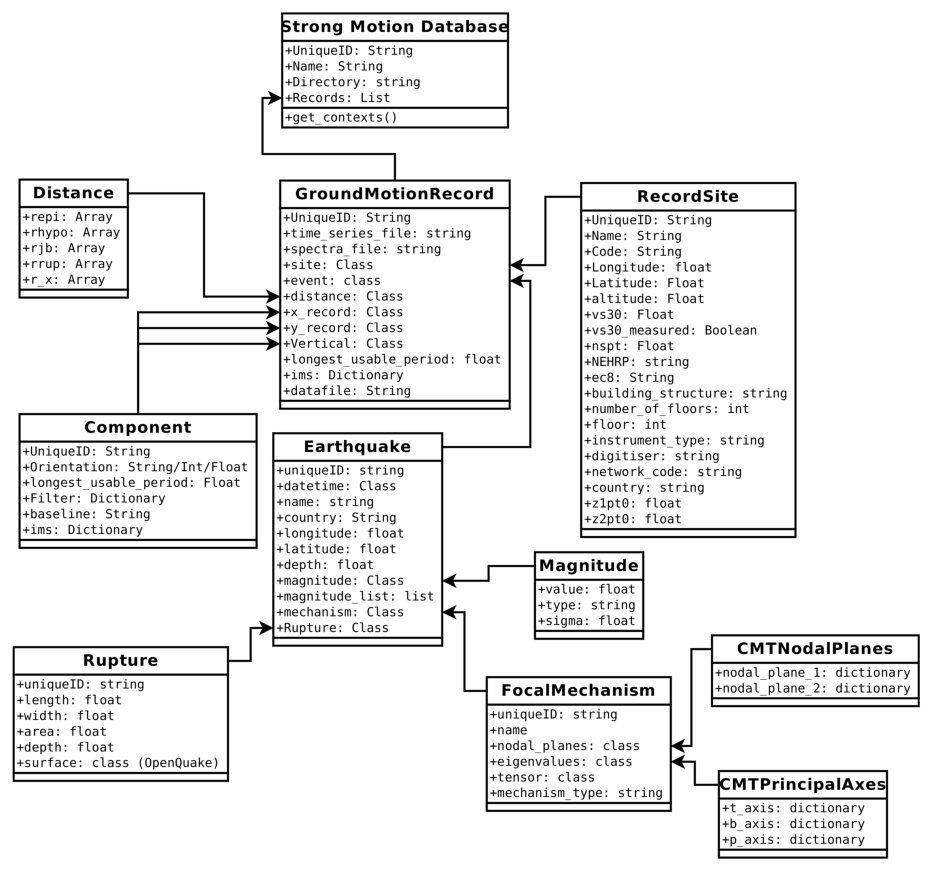
\includegraphics[width=\textwidth]{./figures/database/sm_database_attributes.pdf}
	\caption{Core Architecture of the Strong Motion Data Model}
	\label{fig:sm_data_model}
\end{figure}

The \verb=GroundMotionRecord= class is largely a single container of attributes:
\begin{itemize}
\item \verb=id= Record (waveform) ID
\item \verb=time_series_file=: List of names of the files storing the time series of each of the components of the record.
\item \verb=spectra_file=: List of names of the files storing the response spectra of each of the components of the record (Optional).
\item \verb=event=: Earthquake information as an instance of the \verb=Earthquake= class
\item \verb=distance=: Source to site distance information as an instance of the \verb=RecordDistance= class
\item \verb=site=: Site information as an instance of the \verb=RecordSite= class.
\item \verb=xrecord=: Metadata relating to the first horizontal component of the record as an instance of the class \verb=Component=
\item \verb=yrecord=: Metadata relating to the second horizontal component of the record as an instance of the class \verb=Component=
\item \verb=vertical=: Metadata relating to the vertical component of the record as an instance of the class \verb=Component= (Optional)
\item \verb=average_lup=: Average longest useable period of the record
\item \verb=ims=: Dictionary of scalar intensity measure attributes of the record
\item \verb=datafile=: Location of the processed hdf5 database file for the record.
\end{itemize}


\subsection{Source Characteristics}

The current characterisation of the source is broken down into several different areas: the hypocentre information, magnitude, focal mechanism and finite rupture.

\subsubsection{Earthquake}

The \verb=Earthquake= class contains full characterisation of the event source, with the following attributes:

\begin{itemize}
\item \verb=id=: Unique identifier of the event
\item \verb=datetime=: The date and time of the earthquake as an instance of Python's datetime object. This can be generated as follows:
\begin{python}
from datetime import datetime
# The following event occurs at 2010/6/1 20:36:27.4
event_date_time = datetime(2010, 6, 1, 20, 36, 27, 4E5)
\end{python}
\item \verb=name=: Event Name
\item \verb=country=: Country of event (Optional)
\item \verb=longitude=: Longitude of event (in decimal degrees)
\item \verb=latitude=: Latitude of event (in decimal degrees)
\item \verb=depth=: Hypocentral depth of event (km)
\item \verb=magnitude=: Primary magnitude (usually $M_W$) as instance of the \verb=Magnitude= class
\item \verb=magnitude_list=: Alternative magnitudes for the event, as list of instances of the \verb=Magnitude= class
\item \verb=mechanism=: Earthquake focal mechanism as instance of the \verb=FocalMechanism= class
\item \verb=rupture=: Finite rupture properties as instance of the \verb=Rupture= class
\end{itemize}

In general the preferred magnitude scale is Moment Magnitude $M_W$; however to permit the possibility other scales may be preferred (or for practical purposes assumed equivalent) the \verb=Earthquake= class contains the primary magnitude and a list of other magnitude scales. A magnitude is represented by a separate class called \verb=Magnitude=, which contains the following attributes:

\begin{itemize}
\item \verb=value= The magnitude value
\item \verb=mtype= The magnitude type
\item \verb=sigma= The standard deviation of the magnitude estimate
\end{itemize}

Where possible it is preferable to hold information relating to the focal mechanism of the class. It is anticipated that potentially several components of the focal mechanism may be needed; hence the mechanism is broken down into classes to represent the nodal planes, the eigendecomposition and the moment tensor, all held within the \verb=FocalMechanism= class. This class has the following attributes:
\begin{itemize}
\item \verb=id= Unique identifier (should be different from the event ID)
\item \verb=Name= Focal mechanism name
\item \verb=nodal_planes= The strike dip and rake of the two nodal planes of the focal mechanism as an instance of the class \verb=GCMTNodalPlanes=. This class can be constructed as follows:
\begin{python}
# Two nodal planes: i) Strike = 30., dip = 90., rake = 0.
#                  ii) Strike = 120., dip = 90., rake = 180.
from smtk.sm_database import GCMTNodalPlanes
nps = GCMTNodalPlanes
nps.nodal_plane_1 = {"strike": 30., "dip": 90., "rake" = 0.}
nps.nodal_plane_2 = {"strike": 120., "dip": 90., "rake" = 180.}
\end{python}
 \item \verb=eigenvalues= The eigenvectors (B-, P- and T-) of the principal axes of the mechanism as an instance of the class \verb=GMCTPrincipalAxes=. This can be constructed as follows:
 \begin{python}[frame=single]
 # Mechanism with the following planes
 # T-axis = Eigenvalue 1.5E24, Plunge = 8, Azimuth = 203
 # B-axis = Eigenvalue -0.11E24, Plunge = 77, Azimuth = 332
 # P-axis = Eigenvalue -1.393, Plunge = 10, Azimuth = 111
 from smtk.sm_database import GCMTPrincipalAxes
 pax1 = GCMTPrincipalAxes()
 pax1.t_axis = {"eigenvalue": 1.5E24,
                "azimuth": 203.,
                "plunge": 8.}
 pax1.b_axis = {"eigenvalue": -0.11E24,
                "azimuth": 332.,
                "plunge": 77.}
 pax1.p_axis = {"eigenvalue": -1.393E24,
                "azimuth": 111.,
                "plunge": 10.}
 \end{python}
 \item \verb=tensor= The moment tensor as a $3 \times $ array
 \item \verb=mechanism_type= The style of faulting as a string
\end{itemize}

Finally the \verb=Earthquake= class can contain information relating to the physical dimensions of the rupture (where available!). These are held in the \verb=Rupture= class, with the following attributes:
\begin{itemize}
\item \verb=id=: Unique ID (not the same as the event ID)
\item \verb=length=: Rupture length (km)
\item \verb=width=: Rupture Width (km)
\item \verb=area=: Rupture Area (km$^2$)
\item \verb=depth=: Depth to the top of rupture (km)
\item \verb=surface=: Rupture surface as an instance of the OpenQuake surface class
\end{itemize}


\subsection{Site Characteristics}

In contrast to the \verb=Earthquake= class, all relevant site information is stored in just one class: \verb=RecordSite=. This class contains the following attributes:
\begin{itemize}
\item \verb=id=: Unique station identifier
\item \verb=name=: Station Name
\item \verb=code=: Station Code (as reported by station)
\item \verb=longitude=: Longitude of station
\item \verb=latitude=: Latitude of station
\item \verb=altitude=: Elevation of station (optional)
\item \verb=vs30=: $V_{S30}$ of station
\item \verb=vs30_measured=: Boolean term to indicate if the $V_{S30}$ is measure (True) or inferred (False) (optional)
\item \verb=vs30_measured_type=: Metadata indicating how $V_{S30}$ is measured (optional)
\item \verb=nspt=: Number of hammer blows from standard penetration test (optional)
\item \verb=nehrp=: NEHRP site class (optional)
\item \verb=ec8=: Eurocode 8 site class (optional)
\item \verb=building_structure=: Type of building hosting the recorder (optional)
\item \verb=number_floors=: Number of floors in building hosting the recorder (optional)
\item \verb=floor=: Floor upon which the recorder is situated (optional)
\item \verb=instrument_type=: Type of recording instrument
\item \verb=digitiser=: Type of digitiser
\item \verb=network_code=: Network code
\item \verb=country=: Country of station
\item \verb=z1pt0=: Depth to $V_S$ 1.0 km/s interface (m)
\item \verb=z2pt5=: Depth to $V_S$ 2.5 km/s interface (km)
\end{itemize}

\subsection{Waveform Characteristic}

The database can contain information relating to the manner in which the record has been processed, in addition to other waveform-specific metadata. This information is held in the \verb=Component= class, with the following attributes:
\begin{itemize}
\item \verb=id=: Identifier of the waveform
\item \verb=orientation=: Orientation of the record 
\item \verb=lup=: Longest useable period
\item \verb=filter=: Information about the filter type used. For example, for a ``Butterworth'' filter of 2nd order, with 2 passes and a high and low-cut frequency of 100 Hz and 0.05 Hz respectively, the filter is described via the dictionary:
\begin{python}[frame=single]
filter_data = {"Type": "Butterworth",
               "Order": 2,
               "Passes": 2,
               "Low-Cut": 0.05,
               "High-Cut": 100.0}
\end{python}
Additional data can be added dynamically where necessary
\item \verb=baseline=: Information about baseline adjustment
\item \verb=ims=: Scalar intensity measures of the component.
\item \verb=units=: Units of the waveform
\end{itemize}

\subsection{Geometry Characterisations}

Depending on the information supplied, particularly with respect to the finite rupture, the source-to-site geometry characteristics can be stored in the \verb=RecordDistance= class. In the present form this contains attributes of the five main distance types:

\begin{itemize}
\item \verb=repi=: Epicentral distance (km) from source to site
\item \verb=rhypo=: Hypocentral distance (km)
\item \verb=rjb=: Joyner-Boore distance (km)
\item \verb=rrup=: Rupture distance (km)
\item \verb=r_x=: $R_X$ distance (km)
\end{itemize}

\section{Missing Metadata!}
\label{sec:missing_metadata}

%One of the greatest challenges in construction of a strong motion database is to address the cases where critical (i.e. non-optional) metadata are missing from the record. 

\textbf{TODO - More feedback is needed from users on appropriate methods for obtaining missing metadata!}

\section{The HDF5 Strong Motion Database}
\label{sec:hdf5}

The potentially widespread application of the software requires that the manner in which it is able to create and access waveform data is important to the practical function of the tools. Therefore the decision is made to store the waveforms and related attributes in an \verb=hdf5= database \footnote{\href{http://www.hdfgroup.org/HDF5/}{http://www.hdfgroup.org/HDF5/}}. \verb=hdf5= is a high density binary file format capable of storing data in a nested architecture, allowing large arrays of data (such as waveforms) to be mapped alongside their attributed This database consists of two components. The metadata for each record, mapped according to the \verb=GroundMotionDatabase= class, and the waveform data itself. The waveform data for a database is split into a directory of \verb=hdf5= 
binary files, where each file contains the full waveforms for all three components of the record, as well as the spectra for each waveform, and potentially the horizontally resolved spectra. The full structure of a single ground motion record in a binary format is shown in Figure \ref{fig:sm_hdf5_model}.

\begin{sidewaysfigure}[htbp]
	\centering
		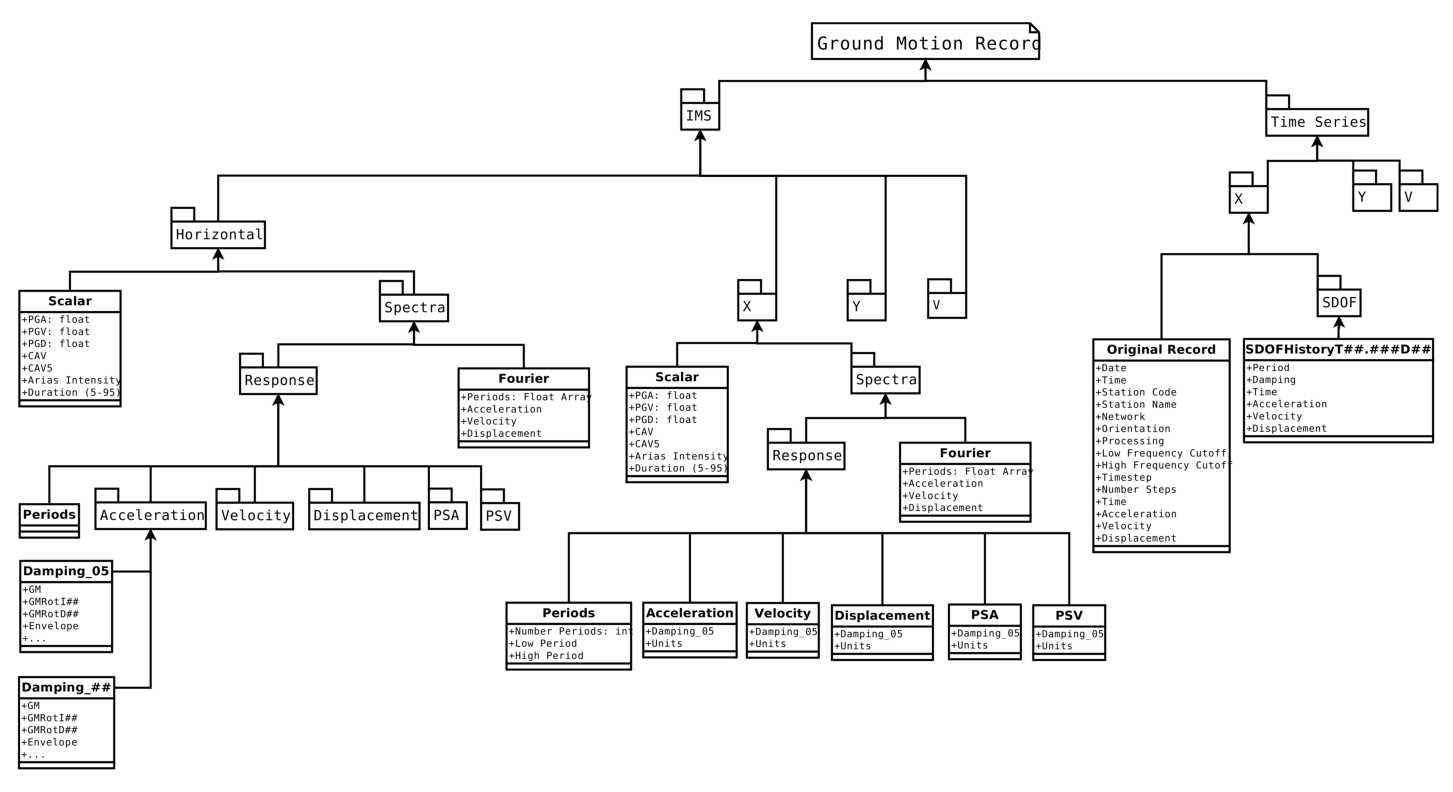
\includegraphics[width=\textwidth]{./figures/database/sm_database_architecture.pdf}
	\caption{Architecture of the hdf5 representation of a strong motion record}
	\label{fig:sm_hdf5_model}
\end{sidewaysfigure}

The \verb=hdf5= format offers several key advantages that have motivated its usage within these tools. Already mentioned was the capability to store large arrays of numerical data in a structure that is conveniently nested in order to associate subsets of data and corresponding attributes. The format is high-density, reducing the overall size of the datafile compared to, for example, plain text ascii format. The file structure is also dynamic allowing for attributes and dataset to be added as needed. This enables the user to undertake the data compilation in several steps, adding on processed data subsequently from the initial compilation stage. The \verb=hdf5= format is widely supported by many different software languages, and its contents visualisable via the cross-platform \verb=HDFView= application \footnote{\href{http://www.hdfgroup.org/products/java/hdfview/}{http://www.hdfgroup.org/products/java/hdfview/}}. 

\subsection{Loading Data to the Database}

In general the creation of a database from a set of records is a process that cannot be readily generalised as each strong motion recording network will define its own data format. Whilst progress is ongoing to add database creators for some of the largest strong motion recording networks, it is necessary for the user to create a customised reader for their own networks. The readers constitute a set of three separate modules, the outline of which can be found in the \verb=smtk.parsers.base_database_parser= module: i) \verb=SMDatabaseReader= the main reader to build the metadata structure of the database (i.e. the \verb=GroundMotionDatabase= class), ii) \verb=SMTimeSeriesReader= to read the waveforms from the respective time series files, and iii) \verb=SMSpectraReader= to read the spectra from files (if provided by the network). If the corresponding database creators are available then a full database can be created using the module \verb=smtk.sm_database_builder.SMDatabaseBuilder=, using the example below:

\begin{python}[frame=single]
# Import the readers for database XXXXX
from smtk.parsers.XXX_database_parser import (XXXMetadataReader,
                                              XXXTimeSeriesReader,
                                              XXXSpectraReader)
# Import the database builder
from smtk.sm_database_builder import SMDatabaseBuilder,

# Path to the directory containing the input files
input_fileset = "./path/to/strong/motion/folder"
# Path to the directory intended for the database
output_database = "./path/to/output/database/folder"

# Create an instance of the database builder
db_builder = SMDatabaseBuilder(XXXMetadataReader,
                               output_database)

# Create the metadata database
db_builder.build_database("UNIQUEID",  # Database ID
                          "DATABASE NAME",  # Name
                          input_fileset)

# Parse the strong motion records
db_builder.parse_records(XXXTimeSeriesReader,
                         XXXSpectraReader)

# (This may take some time if there are many records!!!)
\end{python}
%# If you wish to calculate the resultant horizontal ground motions (e.g. Geometric mean, GMRot etc.)
%# then you can add on this function

%from smtk.sm_database_builder import add_horizontal_im

%intensity_measures = ["PGA", "PGV", "Geometric", "GMRotD50", "GMRotI50"]
%add_horizontal_im(db_builder.database, intensity_measures, component="Geometric", damping="05", periods=[])

The time taken to create the database will obviously depend on many factors, including the number of records and the sampling frequency of each record. For large databases however it could potentially take many hours!

When compiled the database will store the metadata in a file inside the database directory named ``\verb=metadata.pkl=''. This file is a Python binary file (called a ``Pickle'' file or ``pkl'') that stores the \verb=GroundMotionDatabase= class. To load this data into the workspace simply do the following:

\begin{python}[frame=single]
# Import the cPickle module
import cPickle
db1 = cPickle.load(open("path/to/database/metafile.pkl", "r"))
\end{python}


\section{Selecting Subsets of Records from the Database}
\label{sec:sm_selector}

For many of the GMPE tools that will be shown in the rest of this book there will be a frequent need to consider only subsets of the full database. To do this a set of selection tools are created to facilitate the database selection process. These tools can be found in the module \verb=smtk.strong_motion_selector.SMRecordSelector=. To select a subset of the database it is simply necessary to do the following:

\begin{python}[frame=single]
# Import the selector
from smtk.strong_motion_selector import SMRecordSelector
# Create an instance of the class for a specific database
selector = SMRecordSelector(db1)

# Select the 3rd, 6th and 17th record in the database
db2 = selector.select_records([2, 5, 16], as_db=True)
\end{python}

The keyword \verb=as_db= tells the function whether to return the selected records as a new instance of the \verb=GroundMotionDatabase= class. In most cases it is advisable to set this to true, otherwise it will return the selected records as a list of \verb=GroundMotionRecord= classes.

The \verb=SMRecordSelector= has the following selection methods
\begin{itemize}
\item \verb;select_from_record_id(record_id);\\

Selects a record according to its waveform ID.

\item \verb;select_from_event_id(event_id, as_db=False);\\

Returns a set of records from a common event defined by its \verb=event_id=.

\item \verb;select_within_time(start_time=None, end_time=None, as_db=False);\\

Selects records within a specific time window, defined as the interval between \verb=start_time= and \verb=end_time= (both Python datetime objects). For example:

\begin{python}
# Select records between 1990/01/01 and 2010/12/31
db2 = selector.select_within_time(datetime(1990, 1, 1),
                                  datetime(2010, 12, 31),
                                  as_db=True)
\end{python}

\item \verb;select_within_depths(upper_depth=None,;\\
\verb;    lower_depth=None, as_db=False);\\

Selects records corresponding to events within a specific depth range defined as the interval between \verb=upper_depth= (km) and \verb=lower_depth= (km). If not specified \verb=upper_depth= defaults to zero, and lower depth defaults to $\infty$. Records missing a hypocentral depth will not be selected, therefore setting both limits to \verb=None= will effectively filter these records out of the database.

\item \verb;select_within_magnitude(lower=None, upper=None, as_db=False);\\

Select records corresponding to events within a magnitude range, defined as the interval between \verb=lower= (defaults to $-\infty$ if not specified) and \verb=upper= (defaults to $\infty$ if not specified).

\item \verb;select_by_station_country(country, as_db=False);\\

Returns the records within a specific country (input as a string). For example, to select only observations recorded in Italy:

\begin{python}
db2 = selector.select_by_station_country("Italy",
                                         as_db=True)
\end{python}

\item \verb;select_by_site_attribute(attribute, value, as_db=False);\\

Select records corresponding to a particular site attribute (according the attributes listed in the \verb=RecordSite= class). For example to select records only recorded at ``Free-Field'' stations:

\begin{python}
db2 = selector.select_by_site_attribute("building_structure", 
                                        "Free-Field",
                                        as_db=True)
\end{python}

\item \verb;select_within_vs30_range(lower_vs30, upper_vs30, as_db=False);\\

Select records within a given Vs30 range defined as the interval between \verb=lower_vs30= and \verb=upper_vs30=, which default to $-\infty$ and $\infty$ if not specified. As with the depth selection, setting both \verb=lower_vs30= and \verb=upper_vs30= to \verb=None= will remove records missing $V_{S30}$ values from the database. 

\item \verb;select_stations_within_distance(location, distance, as_db=False);\\

Selects records from stations within a distance (km) of a specified location. The location must be input as an instance of an OpenQuake ``Point'' class. For example, to select records within 200 km of $30^{\circ}$E and $40^{\circ}$N:

\begin{python}
from openquake.hazardlib.geo.point import Point
location = Point(30.0, 40.0)
db2 = selector.select_stations_within_distance(location,
                                               200.0,
                                               as_db=True)
\end{python}

\item \verb;select_stations_within_region(region, as_db=False);\\

Selects station inside of a specified region defined by a polygon. The polygon must be input as an instance of the OpenQuake Polygon class. For example, to select all ground motions recorded within a square bounded by $30^{\circ}$E to $40^{\circ}$E and $20^{\circ}$N to $40^{\circ}$N:

\begin{python}
from openquake.hazardlib.geo.point import Point
from openquake.hazardlib.geo.polygon import Polygon

region = Polygon([Point(30.0, 40.0),
                  Point(40.0, 40.0),
                  Point(40.0, 20.0),
                  Point(30.0, 20.0)])
db2 = selector.select_stations_within_region(region,
                                             as_db=True)
\end{python}

\item \verb;select_within_distance_range(distance_type, shortest, furthest,;\\
\verb;    alternative=False, as_db=False);\\
Select records based on a source to site distance range, with the distance type specified by \verb=distance_type=, within the interval \verb=shortest= (defaults to 0 if not specified) and \verb=furthest= (defaults to $\infty$ if not specified). Recognising the possibility that some distance metric may be missing it is possible to also specify a second metric and corresponding distance limits as a tuple via the
\verb=alternative= keyword. For example, select records within a Joyner-Boore distance of 5 km and 50 km, and, if Joyner-Boore distance is not specified select records within an epicentral distance of 10 km and 70 km.

\begin{python}
db2 = selector.select_within_distance_range(
    "rjb", 5.0, 50.0,
    alternative=("repi", 10.0, 70.0),
    as_db=True) 
\end{python}

\item \verb;select_mechanism_type(self, mechanism_type, as_db=False);\\
Select records based on a descriptive event mechanism type. For example, to select records from ``strike-slip'' events:

\begin{python}
db2 = selector.select_mechanism_type("strike-slip",
                                     as_db=True) 
\end{python}

\item \verb;select_event_country(country, as_db=False);\\

Select records corresponding to events whose epicentres occur within a specific country

\item \verb;select_epicentre_within_distance_from_point(location, distance,;\\
\verb;    as_db=False);\\

Selects records from earthquakes whose epicentres are within a distance of a point. The point must be input as an instance of the OpenQuake ``Point'' class.

\item \verb;select_epicentre_within_region(region, as_db=False);\\

Selects records from event inside the specified region. The region must be defined as an instance of the OpenQuake ``Polygon'' class.

\item \verb;select_longest_usable_period(lup, as_db=False);\\

Selects records with a longest usable period greater than or equal to \verb=lup= (in seconds)

\end{itemize}
